

\documentclass[]{report}

\voffset=-1.5cm
\oddsidemargin=0.0cm
\textwidth = 480pt

\usepackage{framed}
\usepackage{subfiles}
\usepackage{graphics}
\usepackage{newlfont}
\usepackage{eurosym}
\usepackage{amsmath,amsthm,amsfonts}
\usepackage{amsmath}
\usepackage{enumerate}
\usepackage{color}
\usepackage{multicol}
\usepackage{amssymb}
\usepackage{multicol}
\usepackage[dvipsnames]{xcolor}
\usepackage{graphicx}
\begin{document}
\subsection*{Question 20}
\begin{itemize}
\item \textbf{\textit{Steal}} is a weakly dominant strategy for
each player and thus \textbf{\textit{(Steal,Steal )}} is a weak dominant-strategy equilibrium.
\begin{figure}[h!]
\centering
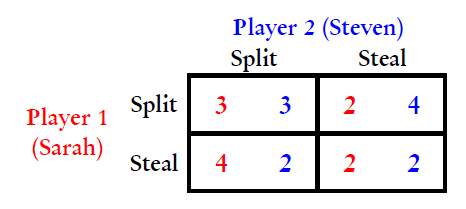
\includegraphics[width=0.55\linewidth]{C:/Users/kevin.obrien/Documents/GitHub/OperationsResearch2/Ramsey/Question20}

\end{figure}


\item \textbf{\textit{Split}} is a strictly dominant strategy for
Player 1, while \textbf{\textit{Steal}} is a weakly (but not strictly) dominant strategy for Player 2
and thus \textbf{\textit{(Split,Steal)}} is a weak dominant-strategy equilibrium.

\begin{figure}[h!]
	\centering
	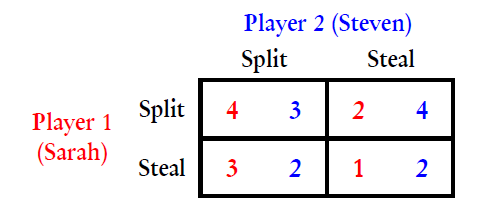
\includegraphics[width=0.55\linewidth]{C:/Users/kevin.obrien/Documents/GitHub/OperationsResearch2/Ramsey/Question20-b}

\end{figure}
\end{itemize}
\end{document}